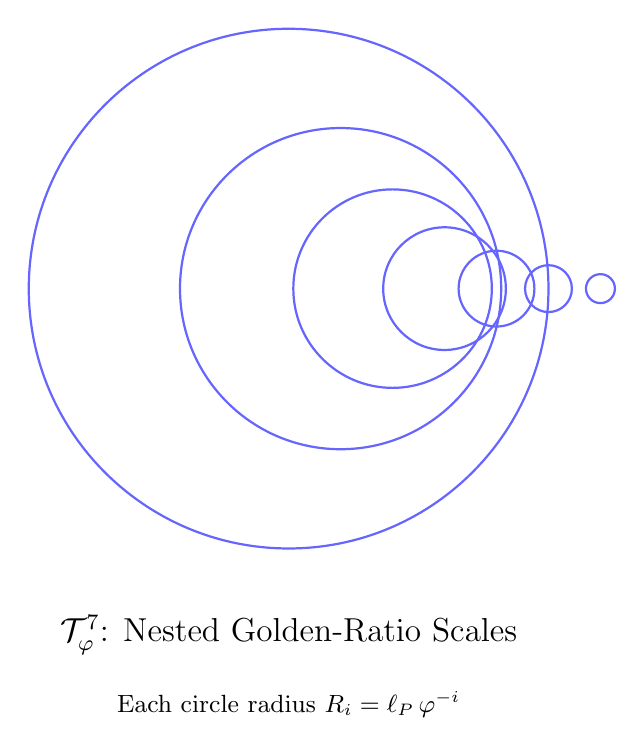
\begin{tikzpicture}[scale=1.1]

% Seven circles with decreasing radii
\foreach \i in {0,...,6} {
    \pgfmathsetmacro{\r}{3*(0.61803398875)^\i}
    \draw[thick,blue!60] (\i*0.6,0) circle (\r cm);
}

\node at (0,-4) {\large $\mathcal{T}^7_{\varphi}$: Nested Golden-Ratio Scales};
\node at (0,-4.8) {\small Each circle radius $R_i = \ell_P\,\varphi^{-i}$};

\end{tikzpicture}
